\documentclass[a4paper,10pt]{article}
\usepackage{graphicx}
\usepackage{lscape}
\usepackage{makecell}
\title{Results}
\author{}
\date{\today}
\begin{document}
\maketitle




\section{Tables of Friedman, Iman-Davendport, Holm-Hochberg and Nemenyi}
\begin{table}[!htp]
\centering
\caption{Comparison and Ranking od METRIC across classifiers}
\resizebox{\textwidth}{!}{%
\begin{tabular}{rllllllll}
Dataset&KNN&Tree&MLP10&RF&SVM&Bayes&GBC&Ada\\
\Xhline{2\arrayrulewidth}
art\_rt&0.732 (4.5)&0.560 (8)&0.712 (7)&0.792 (1)&0.744 (3)&0.768 (2)&0.732 (4.5)&0.728 (6)\\
art\_w\_atleta&0.652 (4)&0.482 (8)&0.680 (3)&0.620 (6)&0.644 (5)&0.704 (2)&0.732 (1)&0.600 (7)\\
art\_w\_braso&0.534 (6.5)&0.534 (6.5)&0.532 (8)&0.580 (4)&0.652 (2)&0.692 (1)&0.644 (3)&0.540 (5)\\
art\_w\_campana&0.618 (7)&0.500 (8)&0.688 (2)&0.658 (6)&0.680 (4)&0.674 (5)&0.684 (3)&0.702 (1)\\
art\_w\_gato&0.646 (5)&0.580 (8)&0.592 (7)&0.660 (4)&0.680 (2)&0.670 (3)&0.692 (1)&0.636 (6)\\
art\_w\_petaka&0.568 (7)&0.550 (8)&0.640 (5)&0.584 (6)&0.692 (1)&0.680 (3)&0.672 (4)&0.688 (2)\\
fon\_rt&0.588 (4)&0.520 (8)&0.528 (7)&0.562 (5)&0.612 (3)&0.548 (6)&0.672 (2)&0.718 (1)\\
fon\_v\_A&0.691 (5)&0.550 (8)&0.738 (1)&0.708 (3.5)&0.721 (2)&0.708 (3.5)&0.686 (6)&0.671 (7)\\
fon\_v\_E&0.660 (6)&0.607 (8)&0.769 (1)&0.735 (3)&0.751 (2)&0.723 (4)&0.644 (7)&0.691 (5)\\
fon\_v\_I&0.639 (7)&0.590 (8)&0.755 (1)&0.702 (4)&0.724 (3)&0.739 (2)&0.668 (5)&0.660 (6)\\
fon\_v\_O&0.683 (3)&0.547 (8)&0.698 (2)&0.673 (5)&0.699 (1)&0.674 (4)&0.650 (6)&0.603 (7)\\
fon\_v\_U&0.724 (6)&0.627 (8)&0.764 (2)&0.732 (5)&0.748 (3.5)&0.773 (1)&0.748 (3.5)&0.719 (7)\\
fon\_w\_atleta&0.595 (5)&0.510 (7)&0.593 (6)&0.614 (3)&0.597 (4)&0.642 (2)&0.666 (1)&0.494 (8)\\
fon\_w\_braso&0.586 (3.5)&0.512 (7)&0.618 (1)&0.584 (5)&0.516 (6)&0.481 (8)&0.615 (2)&0.586 (3.5)\\
fon\_w\_campana&0.746 (2)&0.660 (4)&0.656 (5)&0.636 (7)&0.748 (1)&0.592 (8)&0.724 (3)&0.652 (6)\\
fon\_w\_gato&0.746 (4)&0.608 (8)&0.796 (1)&0.756 (2.5)&0.756 (2.5)&0.696 (6)&0.719 (5)&0.646 (7)\\
fon\_w\_petaka&0.407 (7)&0.485 (1)&0.433 (6)&0.456 (5)&0.484 (2)&0.467 (4)&0.478 (3)&0.400 (8)\\
prs\_rt&0.594 (5)&0.530 (8)&0.592 (6.5)&0.688 (2.5)&0.720 (1)&0.688 (2.5)&0.592 (6.5)&0.600 (4)\\
vggish\_embed\_rt&0.840 (1)&0.490 (8)&0.800 (2)&0.742 (5)&0.768 (4)&0.660 (6)&0.792 (3)&0.632 (7)\\
vggish\_embed\_v\_A&0.750 (3.5)&0.550 (8)&0.784 (2)&0.750 (3.5)&0.746 (5)&0.717 (7)&0.832 (1)&0.736 (6)\\
vggish\_embed\_v\_E&0.661 (6)&0.564 (8)&0.730 (1)&0.684 (4)&0.618 (7)&0.667 (5)&0.700 (3)&0.709 (2)\\
vggish\_embed\_v\_I&0.670 (4)&0.501 (8)&0.710 (1)&0.646 (6)&0.682 (3)&0.652 (5)&0.684 (2)&0.612 (7)\\
vggish\_embed\_v\_O&0.531 (8)&0.585 (5)&0.599 (4)&0.583 (6)&0.650 (1)&0.582 (7)&0.628 (3)&0.632 (2)\\
vggish\_embed\_v\_U&0.655 (3)&0.591 (6)&0.610 (4)&0.595 (5)&0.567 (8)&0.571 (7)&0.679 (1)&0.665 (2)\\
\Xhline{2\arrayrulewidth}
Avg&0.647 (4.88)&0.551 (7.19)&0.667 (3.56)&0.656 (4.46)&0.675 (3.17)&0.657 (4.33)&0.681 (3.31)&0.638 (5.10)\\
\end{tabular}}
\end{table}




\begin{table}[!htp]
\centering
\caption{Best Combinations}
\begin{tabular}{rl|c}
Algorithm&Dataset&AUC\\
\hline
KNN&vggish\_embed\_rt&0.840 \\
GBC&vggish\_embed\_v\_A&0.832 \\
MLP10&vggish\_embed\_rt&0.800 \\
MLP10&fon\_w\_gato&0.796 \\
GBC&vggish\_embed\_rt&0.792 \\
RF&art\_rt&0.792 \\
MLP10&vggish\_embed\_v\_A&0.784 \\
Bayes&fon\_v\_U&0.773 \\
MLP10&fon\_v\_E&0.769 \\
Bayes&art\_rt&0.768 \\
\end{tabular}
\end{table}
\begin{table}[!htp]
\centering
\caption{Average Rankings}
\begin{tabular}{r|l|l}
Algorithm&Ranking&AUC\\
\hline
 SVM & 3.1670 & 0.675 \\
 GBC & 3.3120 & 0.681 \\
 MLP10 & 3.5620 & 0.667 \\
 Bayes & 4.3330 & 0.657 \\
 RF & 4.4580 & 0.656 \\
 KNN & 4.8750 & 0.647 \\
 Ada & 5.1040 & 0.638 \\
 Tree & 7.1880 & 0.551 \\
\end{tabular}
\end{table}




\begin{table}[!htp]
\centering
\caption{Holm-Hochberg}
\begin{tabular}{crcccc}
$i$&algorithm&$z=\frac{R_0 - R_i}{SE}$&$p$&$\alpha/i$&Reject\\
\Xhline{2\arrayrulewidth}
7&Tree (7.19)&5.687e+00&0.000e+00&7.140e-03&\textbf{Reject for SVM} \\
6&Ada (5.10)&2.739e+00&6.160e-03&8.330e-03&\textbf{Reject for SVM} \\
\Xhline{0.5\arrayrulewidth}
5&KNN (4.88)&2.415e+00&1.571e-02&1.000e-02&Not Rejected \\
4&RF (4.46)&1.826e+00&6.789e-02&1.250e-02&Not Rejected \\
3&Bayes (4.33)&1.649e+00&9.915e-02&1.667e-02&Not Rejected \\
2&MLP10 (3.56)&5.586e-01&5.764e-01&2.500e-02&Not Rejected \\
1&GBC (3.31)&2.051e-01&8.375e-01&5.000e-02&Not Rejected \\
\Xhline{2\arrayrulewidth}
\multicolumn{6}{l}{Control method: SVM (3.17)}\\
\multicolumn{6}{l}{Iman Davenport: $F$:9.01 \rightarrow $p-value$:2.316e-09}\\
\end{tabular}
\end{table}




\begin{figure}[!h]
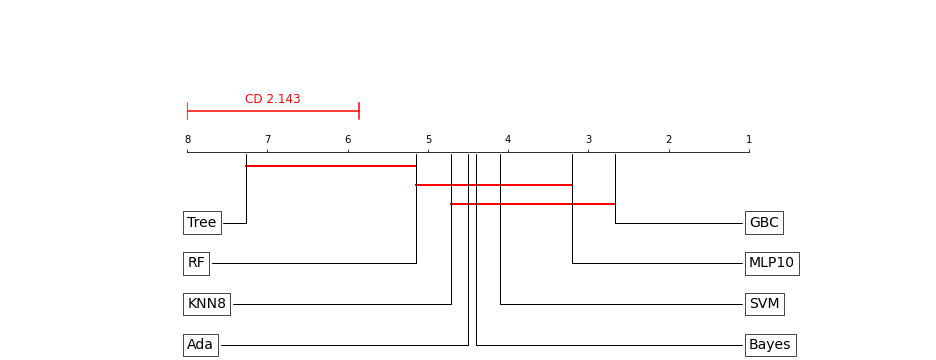
\includegraphics[width=0.95\linewidth]{img/Nemenyi2.png}
\caption{Nemenyi CD diagram}
\label{fig:NemenyiCD}
\end{figure}
\end{document}
